% vim: set ft=plaintex:

\documentclass[]{article}
\usepackage{showlabels}

\usepackage[margin=1in]{geometry}
\usepackage{fancyhdr}
\pagestyle{fancy}

\usepackage{amsmath}
\usepackage{mathtools}
\usepackage{amsfonts}
\usepackage{amssymb}
\usepackage{bbm}

\usepackage{braket}
\usepackage[bold]{hhtensor}
\usepackage{cancel}

\usepackage{amsthm}

% load thmtools but fix "proof proof" bug with thmbox
\usepackage{letltxmacro}
\LetLtxMacro\amsproof\proof
\LetLtxMacro\amsendproof\endproof

\usepackage{thmtools}

\AtBeginDocument{%
  \LetLtxMacro\proof\amsproof
  \LetLtxMacro\endproof\amsendproof
}

\usepackage{nameref,hyperref}
\usepackage[capitalize]{cleveref}

\usepackage{natbib}
\bibliographystyle{humannat}
\usepackage[nottoc]{tocbibind}
\usepackage[toc,page]{appendix}


\usepackage{algorithm2e}
\usepackage{booktabs}
\usepackage{enumitem}
\usepackage{float}
\usepackage{graphicx}
\usepackage[all]{xy}

\usepackage{comment}
\usepackage{todonotes}

% bold \emph
\let\emph\relax
\DeclareTextFontCommand{\emph}{\bfseries\em}

\declaretheorem[thmbox=M]{theorem}
\declaretheorem[thmbox=M,sibling=theorem]{proposition}
\declaretheorem[thmbox=M,sibling=theorem]{lemma}
\declaretheorem[thmbox=M,sibling=theorem]{corollary}
\declaretheorem[thmbox=M,sibling=theorem]{conjecture}
\declaretheorem[
    thmbox={style=M,bodystyle=\normalfont},
    sibling=theorem,
]{definition}
\declaretheorem[
    thmbox={style=M,bodystyle=\normalfont},
    sibling=theorem,
]{example}
\declaretheorem[style=remark,sibling=theorem]{remark}


\makeatletter
\newcommand{\myref}[1]{\cref{#1}\mynameref{#1}{\csname r@#1\endcsname}}
\newcommand{\Myref}[1]{\Cref{#1}\mynameref{#1}{\csname r@#1\endcsname}}
\def\mynameref#1#2{%
  \begingroup
    \edef\@mytxt{#2}%
    \edef\@mytst{\expandafter\@thirdoffive\@mytxt}%
    \ifx\@mytst\empty\else
    \space(\nameref{#1})\fi
  \endgroup
}
\makeatother

\newcommand{\simiid}{\overset{\text{iid}}{\sim}}
\newcommand{\eps}{\varepsilon}
\newcommand{\Rad}{\text{Rad}}


\newcommand{\NN}{\mathbb{N}}
\newcommand{\ZZ}{\mathbb{Z}}
\newcommand{\CC}{\mathbb{C}}
\newcommand{\RR}{\mathbb{R}}
\newcommand{\TT}{\mathbb{T}}
\newcommand{\ind}{\mathbbm{1}}
\newcommand{\fm}{\mathfrak{m}}

\newcommand{\cA}{\mathcal{A}}
\newcommand{\cB}{\mathcal{B}}
\newcommand{\cD}{\mathcal{D}}
\newcommand{\cE}{\mathcal{E}}
\newcommand{\cG}{\mathcal{G}}
\newcommand{\cH}{\mathcal{H}}
\newcommand{\cL}{\mathcal{L}}
\newcommand{\cN}{\mathcal{N}}
\newcommand{\cF}{\mathcal{F}}
\newcommand{\cK}{\mathcal{K}}
\newcommand{\cS}{\mathcal{S}}
\newcommand{\cU}{\mathcal{U}}
\newcommand{\cX}{\mathcal{X}}

\newcommand{\mX}{\matr{X}}
\newcommand{\mY}{\matr{Y}}
\newcommand{\mA}{\matr{A}}
\newcommand{\mB}{\matr{B}}
\newcommand{\mD}{\matr{D}}
\newcommand{\mI}{\matr{I}}
\newcommand{\mK}{\matr{K}}
\newcommand{\mL}{\matr{L}}
\newcommand{\mM}{\matr{M}}
\newcommand{\mP}{\matr{P}}
\newcommand{\mQ}{\matr{Q}}
\newcommand{\mS}{\matr{S}}
\newcommand{\mU}{\matr{U}}
\newcommand{\mV}{\matr{V}}
\newcommand{\mZ}{\matr{Z}}
\newcommand{\mSigma}{\matr{\Sigma}}
\newcommand{\mLambda}{\matr{\Lambda}}
\newcommand{\va}{\vec{a}}
\newcommand{\vb}{\vec{b}}
\newcommand{\vc}{\vec{c}}
\newcommand{\vf}{\vec{f}}
\newcommand{\vg}{\vec{g}}
\newcommand{\vk}{\vec{k}}
\newcommand{\vmu}{\vec{\mu}}
\newcommand{\vp}{\vec{p}}
\newcommand{\vq}{\vec{q}}
\newcommand{\vu}{\vec{u}}
\newcommand{\vw}{\vec{w}}
\newcommand{\vx}{\vec{x}}
\newcommand{\vy}{\vec{y}}
\newcommand{\vz}{\vec{z}}
\newcommand{\vbeta}{\vec{\beta}}
\newcommand{\vsigma}{\vec{\sigma}}
\newcommand{\vxi}{\vec{\xi}}


\DeclareMathOperator{\id}{id}
\DeclareMathOperator{\im}{im}
\DeclareMathOperator{\Ball}{Ball}
\DeclareMathOperator{\Cov}{Cov}
\DeclareMathOperator{\argmax}{argmax}
\DeclareMathOperator{\argmin}{argmin}
\DeclareMathOperator{\diag}{diag}
\DeclareMathOperator{\Var}{Var}
\DeclareMathOperator{\Tr}{Tr}
\DeclareMathOperator{\rank}{rank}
\DeclareMathOperator{\adj}{adj}
\DeclareMathOperator{\TV}{TV}
\DeclareMathOperator{\Vol}{Vol}



\newcommand{\ex}{\mathbb{E}}



\begin{document}

\title{EE290 Course Notes}
\author{Feynman Liang\thanks{\texttt{feynman@berkeley.edu}} \\ Department of Statistics, UC Berkeley}
\date{Last updated: \today}

\maketitle

\tableofcontents


\begin{comment}
\end{comment}

\section{9/5/2019}

\subsection{Results from random matrix theory}

Today we consider random matrices $Z = (Z_{ij}) \in \RR^{n \times n}$.
IID matrix ensemble is when $Z_{ij} \sim P$ are drawn IID, and the
Gaussian Orthogonal Ensemble (GOE) has $Z_{ii} \sim N(0,2)$
and $Z_{ij} = Z_{ji} \sim N(0,1)$ for $i \neq j$.

By convention, normalize and center so $\ex Z_{ij} = 0$ and $\ex Z_{ij}^2 = 1$.

\textbf{Intuition}: $\|Z\|_{op} \leq C \sqrt{n}$ with high probability.

Consider Gaussian orthogonal ensemble matrix: $Z_{ij} \sim N(0,1)$ and $Z_{ii}
\sim N(0,2)$. View $Z = \begin{bmatrix} Z_1, \ldots, Z_n \end{bmatrix}$
with $Z_i \sim N(0, I_n)$. Then
\begin{align}
  \ex \|Z_1\|_2^2 &= \ex[ \sum_{i=1}^n Z_{i1}^2 ] = n \\
  Z_1^\top Z_2 &= \sum_{i=1}^n Z_{i1} Z_{i2} \\
  \ex Z_1^\top Z_2 &= 0 \\
  \ex (Z_1^\top Z_2)^2 &= n \\
  \lvert Z_1^\top Z_2\rvert &\sim \sqrt{n} \\
  \frac{Z_1^\top Z_2}{\|Z_1\| \|Z_2\|} &\sim \frac{1}{\sqrt{n}}
\end{align}

\begin{theorem}[\cite{latala2006estimates}]
  \begin{align}
    \sup_i \sum_{j=1}^n \ex \lvert Z_{ij} \rvert^2 &\leq k^2 n \\
    \sup_j \sum_{i=1}^n \ex \lvert Z_{ij} \rvert^2 &\leq k^2 n
  \end{align}
  Fourth moment bound
  \begin{align}
    \sum_{i=1}^n \sum_{j=1}^n \ex\lvert Z_{ij}\rvert^4 \leq k^4 n^2
  \end{align}

  Then $\ex \|Z\|_{op} = O(k \sqrt{n})$
\end{theorem}

\subsection{Gaussian Orthogonal Ensemble}

$\|Z\|_{op} = \sigma_{max} = \max_{\|v\|=1} v^\top Z v$

For any fixed $v \in S^{n-1}$, we have a Gaussian tail bound
\begin{align}
  v^\top Z v
  &= \sum_i Z_{ii} v_i + \sum_{i < j} 2 Z_{ij} v_i v_j \\
  &= N(0, \sum_i v_i^4 + \sum_{i < j} 4 v_i^2 v_j^2 ) \\
  \Pr(\lvert v^\top Z v \rvert > t) &\leq 2 e^{-t^2 / 4}
\end{align}
Using an $\epsilon$-net, can find a set of vectors $V_{\epsilon}$ such that
\begin{align}
  \max_{v \in V_\epsilon} \lvert v^\top Z v \rvert
  &\geq (1 - 2 \epsilon) \max_{\lvert v \rvert = 1} \lvert z^\top Z v \rvert \geq (1 - 2 \epsilon) t
  \label{eq:eig-eps-net-lb}
\end{align}
Then by a union bound
\begin{align}
  \Pr[ \|Z\|_{op} \geq t ]
  &\leq \Pr[ \max_{v \in V_\epsilon} \lvert v^\top Z v \rvert \geq (1 - 2\epsilon) t ] \\
  &\leq \sum_{v \in V_\epsilon} \Pr[ \lvert v^\top Z v \rvert \geq (1 - 2\epsilon) t ] \\
  &\leq 2 \lvert V \rvert e^{-\frac{1}{4}(1 - 2 \epsilon)^2 t^2} \leq \delta
\end{align}
If $\lvert V \rvert \leq c^n$, then
\begin{align}
  e^{c (n - c t^2)} &\leq e^{\log \delta} \\
  \log \frac{1}{\delta} \leq c t^2 - n &\implies t \geq \sqrt{n + \log \frac{1}{\delta}}
\end{align}

Intuition: when dealing with infinite dimensional maximization (Rayleigh quotient for eigenvalue problem),
can pass to $\epsilon$-net for cardinality bboud.

\begin{definition}[Covering]
  $V \subset S^{n-1}$ is called an $\epsilon$-net if $\forall u \in S^{n-1}$,
  $\exists v \in V$ such that $\|u - v\|_2 \leq \epsilon$.
\end{definition}

\begin{theorem}
  $\epsilon$-net yields \cref{eq:eig-eps-net-lb}
\end{theorem}

\begin{definition}[Packing]
  For $A \subset \RR^d$, $V = \{v_i\}_{i=1}^n \subset A$ is an
  $\epsilon$-packing if $\forall i \neq jJ$, $\| v_i - v_j\|_2 \geq \epsilon$.
\end{definition}

\begin{theorem}
  Maximal $\epsilon$-packing is an $\epsilon$-net.
\end{theorem}

Hence, we can lower bound the packing number (size of largest packing)
by the covering number (size of the smallest covering).
The following result gives an (obvious?) upper bound:

\begin{lemma}[Volume ratio]
  For any $\epsilon$-packing $V \subset A$,
  \begin{align}
    \lvert V \rvert
    \leq \frac{\text{Vol}(A + \frac{\epsilon}{2} B)}{\text{Vol}(\frac{\epsilon}{2} B)}
  \end{align}
  where $B = \{x : \|x\|_2 \leq 1\}$.
\end{lemma}


Why is the diagonal not important? Let $A = \diag(Z)$. Then we have
\begin{align}
  \|Z - A\|_{op}
  &\leq \|Z\|_{op} + \|A\|_{op} \\
  \max_{x \in S^{n-1}} \| A x \| &= \max_i \lvert Z_{ii} \rvert = O(\sqrt{2 \log n})
\end{align}
So the diagonal term $\|A\|_{op}$ is an order of magnitude
smaller that $\|Z\|_{op}$.

\begin{example}[Planted clique]
    Let $G \sim G(1/2, n, k)$. In other words,
    generate an Erd\"os-Renyi random graph from $G(n, 1/2)$ and then
    randomly choose a set $K \subset [n]$ connect together to form a clique.
    
    Goal: find $K$ given $G$.
    
    \begin{theorem}[\cite{alon1998finding}]
      For any $c$, $k = c \sqrt{n}$, then exists polytime algorithm such that
      it returns $\hat{K}$ with $P(\hat{K} = K) \to 1$.
    \end{theorem}
    
    Let the adjacency matrix $A_{ij} = \begin{cases}
        1 & (i,j) \in K \\
        \text{Bern}(1/2) & i \not\in K\text{ or }j \not\in K, i \neq j \\
        0 & i = j
    \end{cases}$ and define $W_{ij} = \begin{cases}
        2 A_{ij} - 1 & i \neq j \\
        0 & i = j
    \end{cases}$
    
    \begin{enumerate}
        \item Find top eigenvector $u$ of $W$
        \item Let $\tilde{K}$ index the $k$ largest coordinates $\lvert u_i \rvert$
        \item  Thresholding
        \begin{align}
            \hat{K} &= \left\{v \in [n] : d_{\tilde{K}}(v) \geq \frac{3k}{4} \right\} \\
            d_{\tilde{K}}(v) &= \sum_{j \in \tilde{K}} \ind\{(j,v) \text{ connected}\}
        \end{align}
    \end{enumerate}
    
    
    Goal: show $\lvert \tilde{K} \cap K \rvert \geq (1 - \epsilon) k$ whp.
    
    Note that $\ex[W] \eqqcolon 1_k 1_k^\top - \diag(1_k)$ consists of $1$s in $K \times K$
    and $0$ everywhere else. Let
    \begin{align}
        W^* &= 1_k 1_k^\top \\
        v &= \frac{1}{\sqrt{k}} 1_k \\
    \end{align}
    Notice thresholding over $v$ exactly recovers $K$, so we want the top
    eigenvector $u$ of $W$ to be close to $v$. By Davis-Kahan,
    \begin{align}
        \min_{s \in \{\pm 1\}} \|u + s v\|_2
        &\leq \frac{\|W - W^*\|_{op}}{\lambda_1(W^*) - \lambda_2(W^*)}
    \end{align}
    Note $\lambda_1(W^*) = k$.
    Suppose extrema attained at $s=-1$, then
    \begin{align}
        \|W - W^*\|_{op} 
        \leq \|W - \ex W\| + \underbrace{\|\ex W - W^*\|}_{=\|\diag 1_k\| = 1}
        \leq c \sqrt{n} + 1
    \end{align}
    
    By Weyl's inequality
    \begin{align}
        \lvert \lambda_2(W) \rvert
        = \lvert \lambda_2(W^*) - \lambda_2(W) \rvert
        \leq \|W^* - W\|_{op}
        \leq c \sqrt{n} + 1
    \end{align}
    Finally
    \begin{align}
        \|u - v\|_2 
        \leq \frac{c \sqrt{n} + 1}{c \sqrt{n} - (c \sqrt{n} + 1)}
        \leq \epsilon
    \end{align}
\end{example}

NOTE: when you have bounded fourth moments, the rate is always $n^{-1/2}$! Deep result.

\section{9/10/2019}

Recall the planted clique from \cite{alon1998finding}: $G \sim G(1/2, n, k)$
is a random graph on $V = [n]$ with some fully connected
clique $K \subset [n]$ of cardinality $\lvert K \rvert = k$.

The adjacency matrix
\begin{align}
  A_{ij} &=
  \begin{cases}
    1 &\text{if }i,j \in K \\
    \text{Bern}(1/2) &\text{$i \neq j$ ow}
  \end{cases}
\end{align}

Let
\begin{align}
    W_{ij} &= \begin{cases}
        2 A_{ij} &\text{if }i \neq j \\
        0 &\text{if }i = j
    \end{cases}
\end{align}
Algorithm 1 of \cite{alon1998finding}:
\begin{enumerate}
    \item Find top eigenvector of $W$, say $u$
    \item Let $\tilde{K}$ index the largest $k$ coordinates $\lvert u_i \rvert$
    \item Define $\hat{K} = \{ v \in V : d_{\tilde{K}}(v) \geq \frac{3 k}{4} \}$
\end{enumerate}

\begin{theorem}[\cite{alon1998finding}]
    Algorithm 1 finds $\hat{K}$ such that $\Pr[\hat{K} = K] \to 1$ as $n \to \infty$
    if $k \geq c \sqrt{n}$ for sufficiently large $c$.
\end{theorem}

\begin{proof}
    Note that $\ex A$ is:
    \begin{figure}[H]
        \centering
        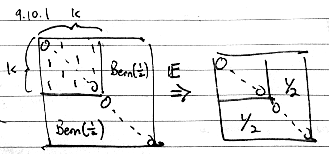
\includegraphics[width=0.6\textwidth]{figures/9-10-1.png}
        \caption{$\ex A$ has ones in the upper $k \times k$ block,
            $0$ on the diagonal, and $1/2$ everywhere else}
    \end{figure}
    
    From this, we can easily see that the $\ex W$ is:
    \begin{figure}[H]
        \centering
        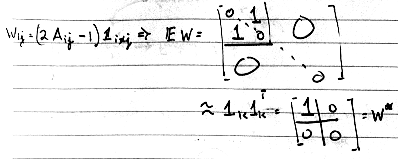
\includegraphics[width=0.6\textwidth]{figures/9-10-2.png}
        \caption{$\ex W$ differs from $W^* = 1_k 1_k^\top$ only in the upper $k$ diagonal}
    \end{figure}
    Note $\ex W = 1_K 1_K^\top - \diag(1_K) \approx 1_K 1_K^\top = W^*$, which
    is good because we have seen that ``differenes in the diagonal are asymptotically negligible.'' \todo{reference for this? 9-5 lecture}
    
    \textbf{Goal}: show $\lvert \tilde{K} \cap K \rvert \geq (1 - \eps) k$ whp, $\eps = \eps(c)$.
    
    We first show the top eigenvector of $W^*$ is close
    to $u$ (the top eigenvector of $W$).
    Let $v = \frac{1}{\sqrt{k}} 1_K$ be the top eigenvector of $W^*$.
    Note $\lambda_1(W^*) = k$.
    By Davis-Kahan
    \begin{align}
        \min_{s \in \{\pm 1\}} \|u + s v\|_2
        &\leq \frac{\|W - W^*\|_{2}}{\lambda_1(w^*) - \lambda_2(w)}
    \end{align}
    Note
    \begin{align}
        \|W - W^*\|
        &\leq \|W - \ex W\| + \|\ex W - W^* \|
        \leq c \sqrt{n} + 1
    \end{align}
    Also $\lambda_1(W^*) = k$ and
    \begin{align}
        \lvert \lambda_2(W) \rvert
        &\leq \lvert \lambda_2(W^*) - \lambda_2(W)
        \leq \|W^* - W\|
    \end{align}
    So by Weyl's inequality
    \begin{align}
        \min_{s \in \{\pm 1\}} \|u + s v\|_2
        &\leq \frac{c \sqrt{n} + 1}{ k - (c \sqrt{n} + 1)} \\
        &\leq \frac{c \sqrt{n} + 1}{c \sqrt{n} - c \sqrt{n} + 1}
        \leq \eps
    \end{align}
        
    Aside: Davis-Kahan to get bound between difference of eigenvectors in 2-norm. Open problem
    to control others.
    
    Next, if $\lvert K \rvert = k = \lvert \tilde{K} \rvert$ then
    $\lvert K \setminus \tilde{K}\rvert = \lvert \tilde{K} \setminus K \rvert$.
    
    \begin{figure}[H]
        \centering
        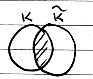
\includegraphics[width=0.2\textwidth]{figures/9-10-3.png}
        \caption{$\lvert K \rvert = \lvert \tilde{K} \rvert \implies \lvert K \setminus \tilde{K} \rvert = \lvert \tilde{K} \setminus K \rvert$ follows from elementary set theory}
    \end{figure}
    
    By definition of $v$
    \begin{align}
        \eps^2
        \geq \|u - v\|_2^2
        = \sum_{i \in K} (u_i - \frac{1}{\sqrt{k}})^2 + \sum_{i \not\in K} u_i^2
    \end{align}
    
    \begin{lemma}
        If all $\lvert u_i \rvert \leq \frac{1}{2 \sqrt{k}}$ for $i \not\in \tilde{K}$, 
        then
        \begin{align}
            \eps^2 
            \geq \sum_{i \in K \setminus \tilde{K}} (\frac{1}{\sqrt{k}} - u_i)^{2} 
            \geq \sum_{i \in K \setminus \tilde{K}} \frac{1}{4k}
        \end{align}
        This implies $\lvert K \setminus \tilde{K} \rvert \leq 4 \eps^2 k$.
    \end{lemma}
    
    \begin{lemma}
        If the condition of the previous lemma does not hold, then $\exists i \in \tilde{K}$
        with $\lvert u_i \rvert \geq \frac{1}{2 \sqrt{k}}$. Then in fact $\lvert u_i \rvert \geq \frac{1}{2 \sqrt{k}}$ for all $i \in \tilde{K}$ since
        \begin{align}
            \eps^2
            &\geq \sum_{i \in \tilde{K} \setminus K} u_i^2
            \geq \sum_{i \in \tilde{K} \setminus K} (\frac{1}{2 \sqrt{k}})^2
            = \sum_{i \in \tilde{K} \setminus K} \frac{1}{4k}
        \end{align}
        Hence $\lvert \tilde{K} \setminus K \rvert \leq 4 \eps^2 k$
    \end{lemma}
    So we have achieved our goal.
    
    To finish the proof, first assume $\|u - v\|_2 \leq \eps$.
    For $a \in K$,
    \begin{align}
        d_{\tilde{K}}(a)
        \geq d_{\tilde{K} \cap K}(a)
        = \lvert \tilde{K} \cap K \rvert - 1
        \geq (1 - \eps') k
    \end{align}
    so for $a \in K$, we will get $a \in \hat{K}$.
    
    Now if $a \not\in K$,
    \begin{align}
        d_{\tilde{K}}(a)
        \leq \underbrace{d_K(a)}_{\sim \text{Binom}(k, 1/2)} + \underbrace{\lvert \tilde{K} \setminus K \rvert}_{\leq \eps' k}
        \approx \frac{k}{2} \pm c \sqrt{k}
    \end{align}
    where $\approx$ means concentration. To be concrete,
    \begin{align}
        \Pr[\hat{K} \neq K]
        &\leq \Pr[\|u - v\|_2 \geq t]
        + \Pr[\exists a \not\in K : d_K(a) \geq (\frac{3}{4} - \eps') k] \\
        &\leq \Pr[ \|W - \ex W\| \geq c \sqrt{n} ]
        + (n - k) \Pr[B(k, 1/2) \geq (\frac{3}{4} - \eps) k] \\
        &\leq c e^{-c' n} + (n - k)
    \end{align}
    
    Where above we used the multiplicative version of Chernoff bound 
    (useful in combinatorial statistics):
    \begin{lemma}[Multiplicative Chernoff Bound]\label{lem:mult-chernoff}
        \begin{align}
            \Pr[X \geq (1 + \delta) \mu]
            &\leq \begin{cases}
                e^{-\delta^2 \mu / 3} &\delta \in [0,1] \\
                e^{-\delta \mu / 3} &\delta \geq 1
            \end{cases} \\
            \Pr[X \leq (1 - \delta) \mu]
            &\leq e^{-\delta^2 \mu / 2}
        \end{align}
    \end{lemma}
    
    As $n \to \infty$, we see that $\Pr[\hat{K} = K] \to 1$.
\end{proof}

\cref{lem:mult-chernoff} is self-normalizing: let $X = \sum_{i=1}^n X_i$ with $X_i$ independent binary
and $\mu = \ex X$. Note that after applying, the RHS does not depend on $n$ \todo{Verify}


\textbf{AKS Algorithm 2}: This algorithm is designed to handle the case when $k$ is not big enough
(recall algorithm 1 requires $k \geq c \sqrt{n}$).
Search over all $S$ with $\lvert S \rvert = C(c) = 2 \log_2 \frac{10}{c} + 2$. For each $S$:
\begin{enumerate}
    \item Define $N^*(S) = \{ v \in V : v \sim a, \forall a \in S \} \setminus S$
    \item Run Algorithm 1 on the induced subgraph (which has distribution $G(1/2, N^*(S), K-S)$),
        return $Q_S \cup S$
    \item Output if $Q_S \cup S$ is a $k$-clique
\end{enumerate}

\textbf{Intuition}: Suppose $k=0$ so there's no clique. Then $\lvert N^*(S) \rvert \sim B(n-s, 2^{-s})
\approx \frac{n-s}{2^s}$ so the total number of nodes is much smaller (by order of $2^{-s}$).
However, the number of clique nodes in $N^*(S)$ is still relatively large, $\geq k - s$.
Solving the critical equation (also for algorithm 1 \todo{Track htis down})
\begin{align}
    k - s \geq C \sqrt{\frac{n}{2^s}}
\end{align}
yields the expression for $C(c)$.


\begin{theorem}
    As long as $k \geq (2 + \eps) \log_2 n$, then exhaustive search finds $k$
    with probability $\to 1$.
\end{theorem}

\begin{proof}
    Exhaustive search will always find the clique, but it may return a clique that we didn't plant.
    So we need to guarantee there is no clique of size $(2 + \eps) \log_2 n$ in $G$ whp.
    
    For $S \subset [n]$, $\lvert S \rvert = k$,
    \begin{align}
        \Pr[S~\text{is clique}] &= \frac{1}{2^{\binom{k}{2}}} \\
        \Pr[\exists S \subset [n] : S~\text{is clique}]
        &\leq \binom{n}{k} \frac{1}{2^{\binom{k}{2}}} 
        \leq (n 2^{-(k-1)/2})^k \to 0\\
    \end{align}
    as $n \to \infty$ ($k = (2 + \eps) \log_2 n$).
\end{proof}
\section{9/12/2019}

\subsection{Planted cliques and semidefinite programming}

Recall the matrix $W$ from before, which has $1$s in the top $k \times k$ block, zero on the diagonal, and $\text{Rad}(1/2)$ RVs elsewhere.

Recall the spectral method:
\begin{align}\label{eq:9-12-orig-spec}
    \hat{u}_{spec} &= \argmax_{\substack{u \in \RR^n \\ \|u\|^2 = k}} u^\top W u
\end{align}
This needs a cleaning step, which we analyzed previously.

How did they come up with this algorithm?
Can we get more insight by analyzing htis method in a more principled framework?
Yes, through maximum likelihood!

Consider an alterantive model where within clique we have connection probability $p$ (instead of $1$) and other connections with probability $q$ (instead of $1/2$),
where $p \gg q$.
\begin{align}\label{eq:9-12-mle}
    \hat{u}_{MLE} &= \argmax_{\substack{u \in \{0,1\}^n \\ \sum_i u_i = k}} u^\top W u
\end{align}

From this, we see that the spectral method is a continuous relaxation of the
MLE integer program. To make this more precise, consider the SDP
\begin{align}\label{eq:9-12-sdp-spec}
    \hat{X}_{spec} &= \argmax_{\substack{X \succeq 0 \\ \Tr X = k}} \braket{W, X}
\end{align}
If we let $X = u u^\top$, then we automatically have $X \succeq 0$ and additionally we have $\Tr X = \|u\|_2^2$. Thus, the feasible set of
\cref{eq:9-12-orig-spec} is the same as \cref{eq:9-12-sdp-spec}.

How do we know the optima of \cref{eq:9-12-sdp-spec} is attained at a rank $1$ matrix
$X = u u^\top$? Since $X = \sum_i \lambda_i u_i u_i^\top$ ($\lambda_i \geq 0$) 
and optima are attained at extremal points, by linearity of $\braket{W,X}$ we can
put all of the weight on a single $\lambda_i$ corresponding to the top eigenvector
of $W$.

How can we get \cref{eq:9-12-sdp-spec} closer to \cref{eq:9-12-mle}? Since
\cref{eq:9-12-mle} is more constrained, we can consider adding more constraints:
\begin{align}\label{eq:9-12-mle-sdp}
    \tilde{X}_{MLE} &= \argmax_X \braket{W, X} \\
    \text{s.t. } & X \succeq 0 \\
                & \Tr X = k \\
                & 0 \leq X \leq J \quad\text{entrywise}\\
                & \braket{X, J} = k^2 \\
                & \rank(X) = 1
\end{align}
where $J = 1 1^\top$.

The solution $X = u u^\top$ where $u \in \{0,1\}^n$, where $u$
indexes the clique.

Conversely, we need to show that the feasible set coincides with \cref{eq:9-12-mle}.
If $X \succeq 0$ and $\rank X = 1$, then we can always write
$X = u u^\top$. The trace constraint now reads $k = \Tr X = \sum_i u_i^2$.
The third constraint becomes $\braket{X, J} = k^2 \implies (\sum_i u_i)^2 = k^2$.

\begin{proposition}
    The optima of \cref{eq:9-12-mle-sdp} must satisfy:
    $u_i \in [-1, 1]$, $\sum u_i^2 = k$, $(\sum_i u_i)^2 = k^2$, 
    $\{u_i\} \in \{0,1\}^n$ or $\{u_i\} \in \{0, -1\}^n$.
    
    In fact, the solution is $u = 1_k$ or $u = -1_k$.
\end{proposition}

The linear constraints in \cref{eq:9-12-mle-sdp} are fine, but the rank constraints
are difficult.
Here is an easier candidate SDP:
\begin{align}\label{eq:9-12-mle-sdp-relax}
    \hat{X}_{SDP} &= \argmax_X \braket{W, X} \\
    \text{s.t. } & X \preceq 0 \\
                 & X \geq 0 \\
                 & \Tr X = k \\
                 & \braket{X, J} = k^2
\end{align}
Notice we have dropped the rank constraint as well as the upper entrywise bound.

\begin{theorem}
    $\exists c > 0$ such that for $k \geq c \sqrt{n}$, \cref{eq:9-12-mle-sdp-relax}
    has unique maximizer $X^* = 1_k 1_k^\top$ with high probability.
\end{theorem}

\begin{proof}
    We first show $X^*$ is a maximizer.
    \begin{align}
        \braket{W, X^*} &= 1_k^\top W 1_k = k^2 - k \\
        \braket{W, X} &= \braket{W + I, X} - \Tr X \\
        \Tr(I - X) = \Tr X &\leq \braket{J, X} - \Tr(X) \\
        \underbrace{W + I \leq J}_{X \geq 0} &\implies \braket{J, X} \geq \braket{W + I, X} \\
        \therefore \Tr(I - X) = \Tr X &\leq k^2 - k
    \end{align}
    
    The harder part is uniqueness. We will develop a general technique called
    dual certificate / KKT condition.
    Write the Lagrangian for the optimization problem.
    Introduce dual variables $S \succeq 0$, $B \geq 0$,
    $\eta \in \RR$, $\lambda \in \RR$ and 
    \begin{align}
        \cL(X, S, B, \eta, \lambda)
        &= \braket{W, X} + \braket{S, X} + \braket{B, X} + \eta\left(
            k \Tr(X) + \lambda (k^2 - \braket{X, J}
        \right)
    \end{align}
    Notice
    \begin{align}
        \max_{X\text{ feas}} \braket{W, X} &= \max_X \min_{S, B, \eta, \lambda} \cL
    \end{align}
    as desired. Since $\cL$ is linear, by Sion's minimax theorem we have
    \begin{align}
        \max_X \min_{S, B, \eta, \lambda} \cL
        &= \min_{S, B, \eta, \lambda} \max_X \cL
    \end{align}
    Note $\braket{S,X} = \Tr( S^{1/2} X S^{1/2} ) \geq 0$ is non-negative.
    $\braket{B, X}$ is also trivially non-negative.
    
    \begin{lemma}\label{lem:x-star-unique-maximizer}
        The following conditions imply $X^*$ is the unique maximizer:
        \begin{enumerate}
            \item Stationarity: $W + S + B - \eta I - \lambda J = 0$ (can't improve any more)
            \item Primal/dual feasibility
            \item Complementary slackness: $\braket{S, X^*} = 0$ and $\braket{B, X^*} = 0$.
            \item Uniqueness: $\lambda_{n-1}(S) > 0$ (second smallest eigenvalue of $S$)
        \end{enumerate}
        The first three conditions are the ``KKT conditions.'' Together,
        they guarantee $X$ is a maximizer.
    \end{lemma}
    
    \begin{proof}[Proof of \cref{lem:x-star-unique-maximizer}]
        \textbf{$X^*$ is a maximizer}: for feasible variables
        \begin{align}
            \braket{W, X} &\leq \cL(X, S, B, \eta, \lambda) &&\text{feasible} \\
            &= \cL(X^*, S, B, \eta, \lambda) &&\text{stationarity} \\
            &= \braket{W, X^*} &&\text{comp. slackness}
        \end{align}
        
        \textbf{Uniqueness}: Suppose $X'$ satisfies $\braket{W, X'} = \braket{W, X^*}$.
        Then $\braket{S, X'} = 0$, and
        $\braket{S, X^*} = 0 \implies 1_k^\top S 1_k = 0 \implies S 1_k = 0$.
        In other words, $1_k$ is an eignevector with eigenvalue $0$ for $S$.
        But condition (4) means that $1_k$ is the only eigenvector with eigenvalue
        $0$, hence $X' = c X^*$ for some $c \in \RR$. But by the
        constrant $\Tr X = k$, we must have $X' = X^*$.
    \end{proof}
    
    Hence, if we can find $(S, B, \eta, \lambda)$ satisfying \cref{lem:x-star-unique-maximizer}, then we have a certificate that
    $X^*$ is the unique maximizer.
    
    But how can we find this certificate? It's hard in general, but in this
    case we have an explicit construction.
    \begin{align}
        B \geq 0, \quad \eta \in \RR, \quad \lambda \in \RR \\
        S = \eta I + \lambda J - B - W \succeq 0 \\
        S 1_k = 0, \quad \braket{B, X^*} = 0, \quad \lambda_{n-1}(S) > 0 \label{eq:9-12-star}
    \end{align}
    \begin{align}
        S 1_k = 0 \implies \eta I_k + \lambda k 1 = B 1_k + W 1_k
    \end{align}
    $X^* = 1_k 1_k^\top$. Since we want $\braket{B, X^*} = 0$, we want
    $B_{ij} = 0$ for $(i,j) \in K \times K$.
    This implies that $(B 1_k)i = 0$ for $i \in K$.
    Let $y = W 1_k$.
    
    $i$th entry, $i \in K$, of \cref{eq:9-12-star} implies $\eta + k \lambda = (B 1_k)_i + y_i = k-1$. Then, choose $\eta = k - 1 - k \lambda$
    
    Now for $i \not\in K$, \cref{eq:9-12-star} implies $\lambda k = (B 1_k)_i + y_i$.
    Construct $B = 1_k b^\top + b 1_k^\top$ for some $b \in \RR^n$ such
    that $b_i = 0$ for $i \in K$.
    Then $B 1_k = k b$.
    
    Fig 9.12.1
    
    $b_i = \lambda - \frac{y_i}{k}$ for all $i \not\in k$.
    Check $B \geq 0 \implies b_i \geq 0$. Since $\lambda \geq \frac{y_i}{k}$ for all
    $i \in K$, $\lambda \geq \max_{i \not\in K} \frac{y_i}{k}$.
    $y_i = W 1_k$ which is a sum of $\text{Rad}(1/2)$ RVs, so 
    by concentration for some $\lambda \geq c$ this is satisfied whp.
    
    For the last part, we need to show $x^\top S x > 0$ for all $x$ such that
    $x^\top 1_k = 0$. The exact formula for $S$ is 
    \begin{align}
        S 
        &= \eta + \underbrace{\lambda x^\top J x}_{\geq O(\sqrt{n})} - \underbrace{x^\top B x}_{=0} - \underbrace{x^\top W x}_{\geq O(\sqrt{n})} \\
        &\geq \frac{k}{2} - 1 - x^\top \ex[W] x - \|W - \ex W\|_{op} \\
        &\geq 0 &&\text{for suff large $k$}
    \end{align}
\end{proof}

\bibliography{refs.bib}

\end{document}
